% ==========================================================================
%  Which screw drive?  --  one 16:9 slide: every drive placed by who can open it
%  (across) and how well the bit grips (up). Same palette and type as the other posters.
%  Compile: just
% ==========================================================================
\RequirePackage{fix-cm}
\documentclass{article}
\usepackage[paperwidth=600mm,paperheight=337.5mm,left=16mm,right=16mm,top=12mm,bottom=12mm]{geometry}
\usepackage[utf8]{inputenc}
\usepackage[T1]{fontenc}
\usepackage[sc]{mathpazo}          % Palatino text + math
\linespread{1.05}
\usepackage{textcomp}
\usepackage{pifont}
\usepackage{xcolor}
\usepackage{tikz}
\usetikzlibrary{calc}
\usepackage[hidelinks]{hyperref}

\pagestyle{empty}
\setlength{\parindent}{0pt}
\frenchspacing

% ---------------- palette ----------------
\definecolor{paper}{HTML}{F8F5EE}
\definecolor{ink}{HTML}{1E2430}
\definecolor{accent}{HTML}{1F4E79}
\definecolor{accentlt}{HTML}{6E93B5}
\definecolor{trap}{HTML}{9A3B2E}
\definecolor{muted}{HTML}{6B7280}
\definecolor{rule}{HTML}{B9C6D3}
\definecolor{good}{HTML}{3C7A4A}
\definecolor{steel}{HTML}{D9DEE4}
\definecolor{empty}{HTML}{EFEBE2}
\definecolor{copper}{HTML}{C27C4E}
\pagecolor{paper}
\color{ink}

\newcommand{\repourl}{https://github.com/samo4/ee-posters}

% ---------------- screw heads, seen from above, on a unit disc ----------------
\tikzset{head/.style={fill=steel, draw=muted, line width=1.2pt},
         recess/.style={fill=ink, draw=none}}
\newcommand{\headdisc}{\draw[head] (0,0) circle (1);}
% #1 lobes, #2 radius
\newcommand{\lobes}[2]{plot[smooth cycle, domain=0:{360-360/#1/10}, samples={10*#1}]
  (\x:{#2*(0.8+0.2*cos(#1*\x))})}
\newcommand{\cross}[2]{% #1 half-width at the tips, #2 reach
  (#1,#1) -- (#1,#2) -- (-#1,#2) -- (-#1,#1) -- (-#2,#1) -- (-#2,-#1)
  -- (-#1,-#1) -- (-#1,-#2) -- (#1,-#2) -- (#1,-#1) -- (#2,-#1) -- (#2,#1) -- cycle}
\newcommand{\pzticks}{\foreach \a in {45,135,225,315} \draw[ink, line width=1.4pt] (\a:0) -- (\a:0.66);}

\newcommand{\iconslotted}{\headdisc \fill[recess] (-0.92,-0.1) rectangle (0.92,0.1);}
\newcommand{\iconcombo}{\headdisc \pzticks
  \fill[recess] (-0.92,-0.09) rectangle (0.92,0.09);
  \fill[recess] \cross{0.09}{0.55}; \fill[recess, rotate=45] (-0.16,-0.16) rectangle (0.16,0.16);}
\newcommand{\iconphillips}{\headdisc
  \fill[recess, rounded corners=0.6pt] \cross{0.11}{0.62}; \fill[recess] (0,0) circle (0.2);}
\newcommand{\iconpozidriv}{\headdisc \pzticks
  \fill[recess] \cross{0.09}{0.62}; \fill[recess, rotate=45] (-0.17,-0.17) rectangle (0.17,0.17);}
\newcommand{\iconrobertson}{\headdisc \fill[recess] (-0.36,-0.36) rectangle (0.36,0.36);}
\newcommand{\icontorx}{\headdisc \fill[recess] \lobes{6}{0.55};}
\newcommand{\iconhex}{\headdisc
  \fill[recess] (0:0.55) -- (60:0.55) -- (120:0.55) -- (180:0.55) -- (240:0.55) -- (300:0.55) -- cycle;}
\newcommand{\iconpentalobe}{\headdisc \fill[recess] \lobes{5}{0.5};}
\newcommand{\icontriwing}{\headdisc
  \foreach \a in {90,210,330} \fill[recess, rotate=\a] (0,-0.13) -- (0.62,-0.02) -- (0.62,0.18) -- (0,0.13) -- cycle;
  \fill[recess] (0,0) circle (0.16);}
\newcommand{\icontorxsec}{\headdisc \fill[recess] \lobes{6}{0.55};
  \fill[steel] (0,0) circle (0.16); \draw[muted, line width=0.8pt] (0,0) circle (0.16);}
\newcommand{\iconspanner}{\headdisc \fill[recess] (-0.45,0) circle (0.13) (0.45,0) circle (0.13);}
% drives on the outside: the head itself is the shape, the tool wraps around it
\newcommand{\hexagon}[1]{(0:#1) -- (60:#1) -- (120:#1) -- (180:#1) -- (240:#1) -- (300:#1) -- cycle}
\newcommand{\iconthumb}{\headdisc
  \foreach \a in {0,10,...,350} \draw[muted, line width=1pt] (\a:0.82) -- (\a:1);
  \draw[muted, line width=0.8pt] (0,0) circle (0.82);}
\newcommand{\iconhexhead}{\draw[head, rotate=30] \hexagon{1}; \draw[muted, line width=0.8pt] (0,0) circle (0.8);}
\newcommand{\iconetorx}{\draw[head] plot[smooth cycle, domain=0:354, samples=60] (\x:{0.9+0.1*cos(6*\x)});
  \draw[muted, line width=0.8pt] (0,0) circle (0.62);}
% joints that never come apart
\newcommand{\iconweld}{\draw[head] (-1,-0.75) rectangle (1,0.75);
  \fill[muted!45] (-0.24,-0.75) rectangle (0.24,0.75);
  \foreach \y in {-0.62,-0.44,...,0.6} \draw[muted, line width=0.9pt] (-0.24,\y) .. controls (0,\y+0.14) .. (0.24,\y);}
\newcommand{\iconrivet}{\shade[ball color=steel] (0,0) circle (1); \draw[muted, line width=1.2pt] (0,0) circle (1);}
\newcommand{\iconcrimp}{\draw[head] (-0.45,0) circle (0.5); \draw[muted, line width=1.2pt, fill=white] (-0.45,0) circle (0.2);
  \fill[copper] (0.8,-0.12) rectangle (1.1,0.12);
  \draw[head] (-0.02,-0.24) rectangle (0.85,0.24);
  \foreach \x in {0.3,0.55} \draw[ink, line width=1.6pt] (\x,-0.24) -- (\x,0.24);}
\newcommand{\iconsolder}{\draw[fill=copper, draw=copper!70!black, line width=1.2pt] (0,0) circle (0.95);
  \shade[ball color=steel] (0,0) circle (0.66); \fill[muted] (0,0) circle (0.17);}
\newcommand{\iconglue}{\draw[head] (0,0.95) .. controls (0.15,0.5) and (0.7,0.1) .. (0.7,-0.25)
  arc (0:-180:0.7) .. controls (-0.7,0.1) and (-0.15,0.5) .. (0,0.95) -- cycle;
  \fill[white] (-0.32,-0.3) ellipse (0.1 and 0.18);}
% a left-hand nut from above: notches cut into every corner, and it tightens anticlockwise
\newcommand{\iconthread}{%
  \draw[head] \hexagon{0.95};
  \foreach \a in {0,60,...,300} {
    \coordinate (p) at ($(\a:0.95)!0.17!(\a-60:0.95)$);
    \coordinate (q) at ($(\a:0.95)!0.17!(\a+60:0.95)$);
    \fill[white] (p) -- (\a:0.97) -- (q) -- (\a:0.7) -- cycle;
    \draw[muted, line width=1.2pt, line join=round] (p) -- (\a:0.7) -- (q);}
  \draw[muted, line width=0.8pt, fill=white] (0,0) circle (0.38);
  \draw[ink, line width=0.8pt] (0:0.48) arc (0:270:0.48);
  \draw[trap, line width=1.8pt, -stealth] (40:1.2) arc (40:140:1.2);}

% ---------------- the grid ----------------
\newcommand{\cellw}{138.4}
\newcommand{\cellh}{44}
\newcommand{\gap}{4.5}
% (\ax,\ay): #3, #4 mm right of and above the south-west corner of cell #1 (column 0..3), #2 (row 0..4 from the bottom)
\newcommand{\at}[4]{\pgfmathsetmacro\ax{#1*(\cellw+\gap)+#3}\pgfmathsetmacro\ay{#2*(\cellh+\gap)+#4}}

\tikzset{cell/.style={fill=white, draw=rule, line width=1.2pt, rounded corners=4mm},
         vacant/.style={fill=empty, draw=none, rounded corners=4mm}}
\newcommand{\pro}[1]{\hangindent=1.15em\hangafter=1\makebox[1.15em][l]{\color{good}\upshape\ding{51}}#1\par}
\newcommand{\con}[1]{\hangindent=1.15em\hangafter=1\makebox[1.15em][l]{\color{trap}\upshape\ding{55}}#1\par}
% [#1] cell style, #2 column, #3 row, #4 icon, #5 name, #6 why use it, #7 why not
\newcommand{\drive}[7][]{%
  \at{#2}{#3}{0}{0}\draw[cell, #1] (\ax,\ay) rectangle ++(\cellw,\cellh);
  \at{#2}{#3}{17}{\cellh/2}\begin{scope}[shift={(\ax,\ay)}, scale=12.5]#4\end{scope}
  \at{#2}{#3}{34}{\cellh/2}\node[anchor=west, text width={(\cellw-37)*1mm}, align=left, inner sep=0pt]
    at (\ax,\ay)
    {\spaceskip=0pt \xspaceskip=0pt \hyphenpenalty=10000 % align=left fixes spaces at .3333em of the 10pt font
     {\fontsize{30}{33}\selectfont\bfseries #5\par}\vspace{1.5mm}
     {\fontsize{18.5}{22}\selectfont\itshape \pro{#6}\con{#7}}};}
\newcommand{\vacant}[2]{\at{#1}{#2}{0}{0}\fill[vacant] (\ax,\ay) rectangle ++(\cellw,\cellh);}

\begin{document}
\noindent
\begin{minipage}[t][\dimexpr\textheight-\topskip-1mm\relax][s]{\linewidth}\vspace{0pt}
% ===================================================================== title
{\fontsize{80}{84}\selectfont\bfseries Which screw drive?}\hfill
{\fontsize{28}{34}\selectfont\itshape\color{muted}Start at Torx. Amen.}\par
\vspace{3mm}
{\color{accent}\rule{\linewidth}{2.5pt}}\par
\vfill
% ===================================================================== the grid
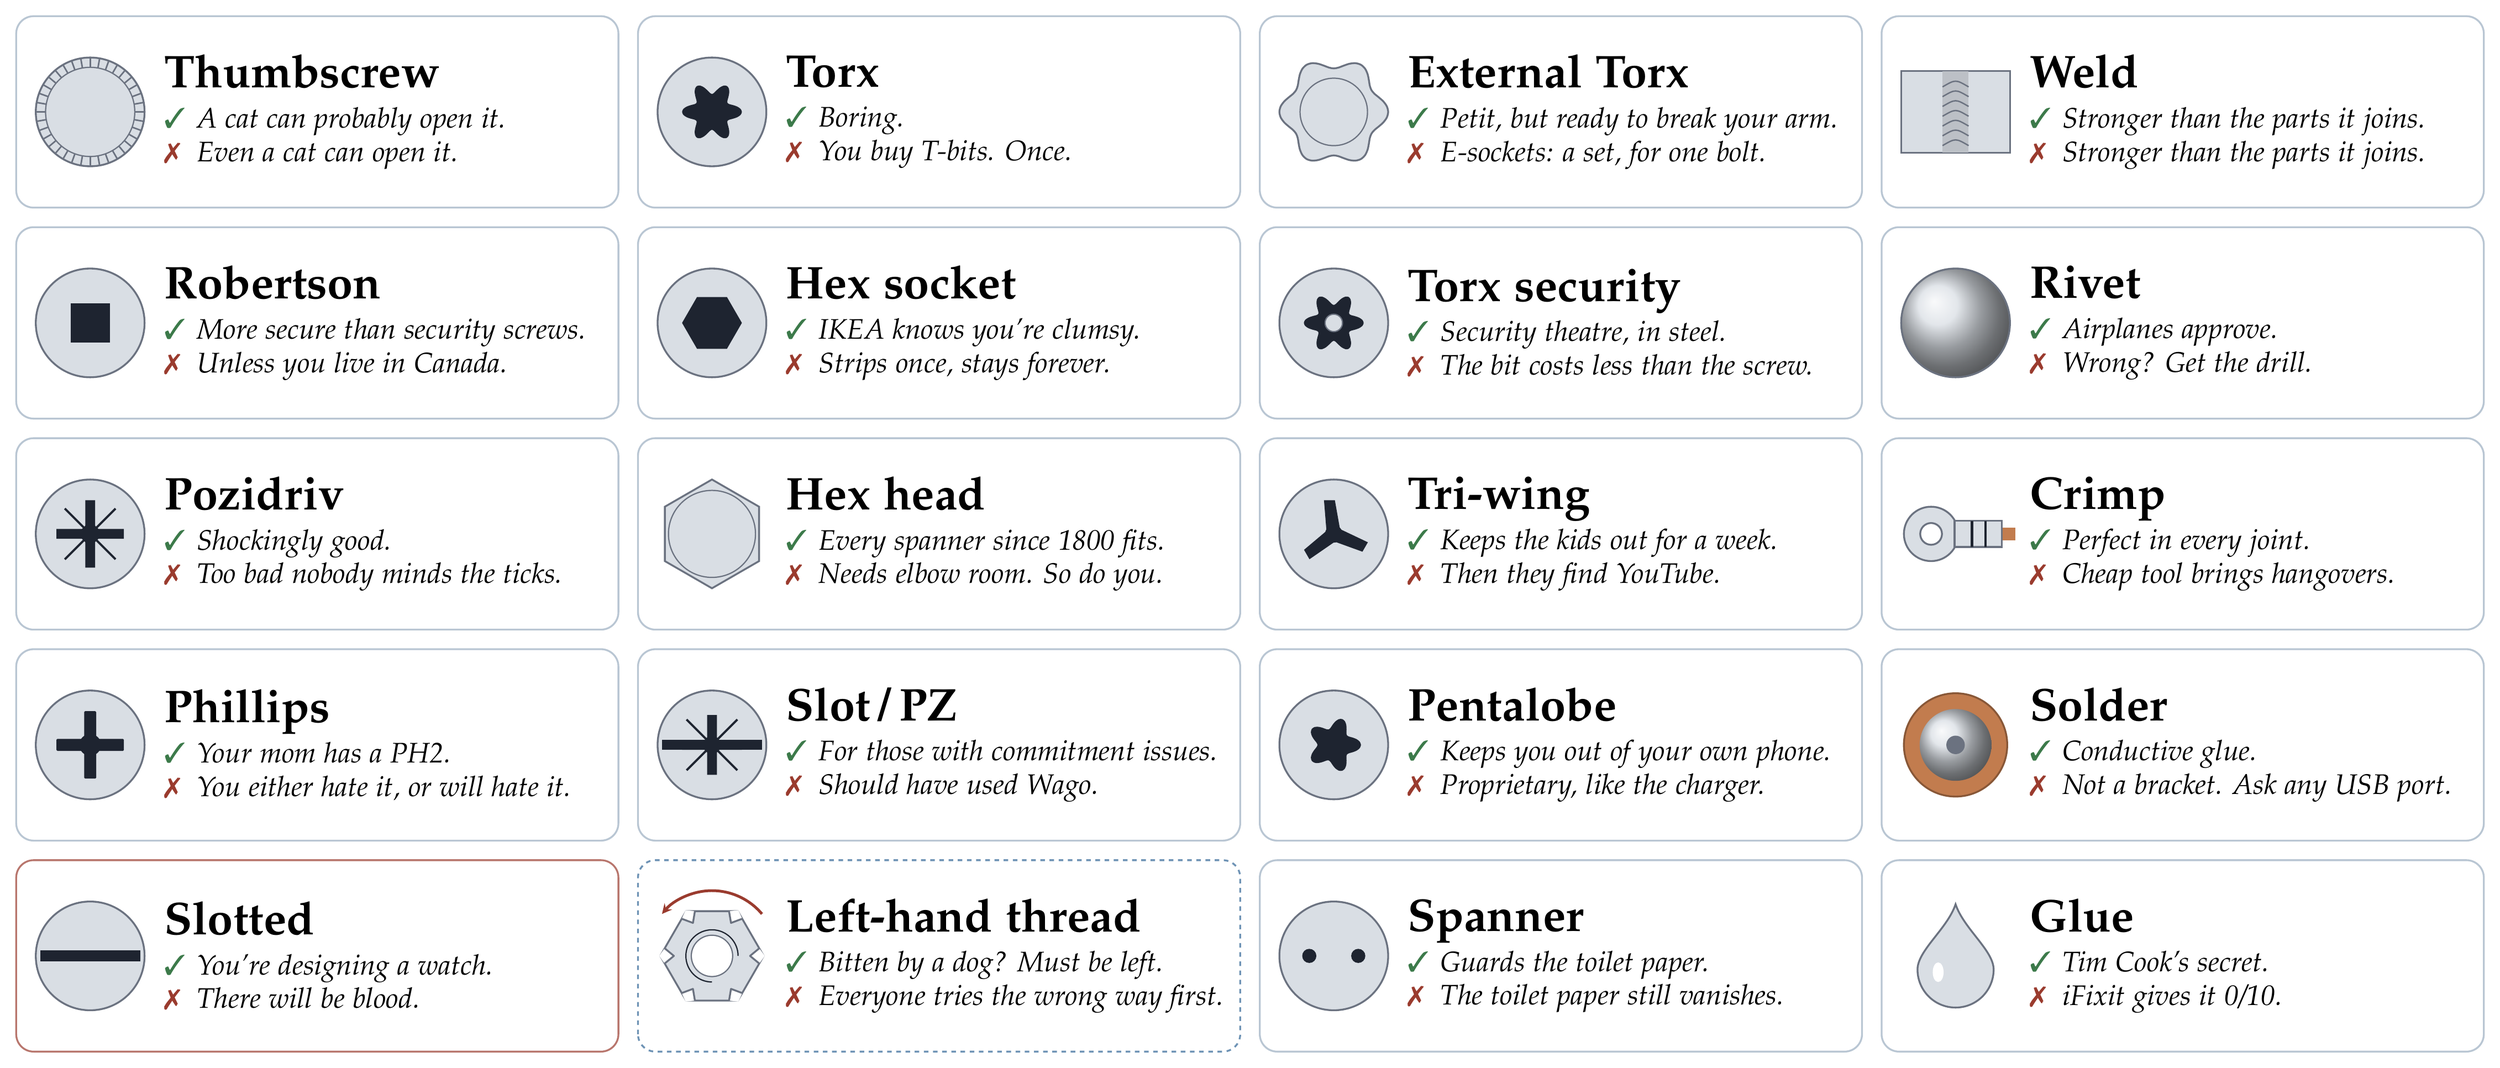
\begin{tikzpicture}[x=1mm, y=1mm]
  % ---- anyone
  \drive{0}{4}{\iconthumb}{Thumbscrew}
    {A cat can probably open it.}
    {Even a cat can open it.}
  \drive{0}{3}{\iconrobertson}{Robertson}
    {More secure than security screws.}
    {Unless you live in Canada.}
  \drive{0}{2}{\iconpozidriv}{Pozidriv}
    {Shockingly good.}
    {Too bad nobody minds the ticks.}
  \drive{0}{1}{\iconphillips}{Phillips}
    {Your mom has a PH2.}
    {You either hate it, or will hate it.}
  \drive[draw=trap!70]{0}{0}{\iconslotted}{Slotted}
    {You're designing a watch.}
    {There will be blood.}
  % ---- any toolbox
  \drive{1}{4}{\icontorx}{Torx}
    {Boring.}
    {You buy T-bits. Once.}
  \drive{1}{3}{\iconhex}{Hex socket}
    {IKEA knows you're clumsy.}
    {Strips once, stays forever.}
  \drive{1}{2}{\iconhexhead}{Hex head}
    {Every spanner since 1800 fits.}
    {Needs elbow room. So do you.}
  \drive{1}{1}{\iconcombo}{Slot\,/\,PZ}
    {For those with commitment issues.}
    {Should have used Wago.}
  \drive[dashed, draw=accentlt]{1}{0}{\iconthread}{Left-hand thread}
    {Bitten by a dog? Must be left.}
    {Everyone tries the wrong way first.}
  % ---- a 10 euro bit set
  \drive{2}{4}{\iconetorx}{External Torx}
    {Petit, but ready to break your arm.}
    {E-sockets: a set, for one bolt.}
  \drive{2}{3}{\icontorxsec}{Torx security}
    {Security theatre, in steel.}
    {The bit costs less than the screw.}
  \drive{2}{2}{\icontriwing}{Tri-wing}
    {Keeps the kids out for a week.}
    {Then they find YouTube.}
  \drive{2}{1}{\iconpentalobe}{Pentalobe}
    {Keeps you out of your own phone.}
    {Proprietary, like the charger.}
  \drive{2}{0}{\iconspanner}{Spanner}
    {Guards the toilet paper.}
    {The toilet paper still vanishes.}
  % ---- never comes apart
  \drive{3}{4}{\iconweld}{Weld}
    {Stronger than the parts it joins.}
    {Stronger than the parts it joins.}
  \drive{3}{3}{\iconrivet}{Rivet}
    {Airplanes approve.}
    {Wrong? Get the drill.}
  \drive{3}{2}{\iconcrimp}{Crimp}
    {Perfect in every joint.}
    {Cheap tool brings hangovers.}
  \drive{3}{1}{\iconsolder}{Solder}
    {Conductive glue.}
    {Not a bracket. Ask any USB port.}
  \drive{3}{0}{\iconglue}{Glue}
    {Tim Cook's secret.}
    {iFixit gives it 0/10.}
\end{tikzpicture}\par
\vfill
% ===================================================================== footer
{\color{rule}\rule{\linewidth}{0.8pt}}\par\vspace{3mm}
{\fontsize{28}{32}\selectfont\itshape Somebody will open it. Choose who.}\hfill
{\fontsize{15}{18}\selectfont\href{\repourl}{\color{muted}\repourl}}\par
\end{minipage}
\end{document}
